% LuaLaTeX文書; 文字コードはUTF-8
\documentclass[17pt]{beamer}% 'unicode'が必要
\usepackage{luatexja-fontspec}
\newjfontface{\nonproportional}{BIZ UDMincho}[YokoFeatures={JFM=ujis}]
\setmainjfont[Ligatures={Common,TeX},
  ItalicFont={BIZ UDPMincho},
  ItalicFeatures={FakeSlant=0.27},
  SlantedFont={BIZ UDPMincho},
  SlantedFeatures={FakeSlant=0.18},
  BoldFont={BIZ UDPGothic Bold},
  BoldSlantedFont={BIZ UDPGothic Bold},
  BoldSlantedFeatures={FakeSlant=0.18},
  BoldItalicFont={BIZ UDPGothic Bold},
  BoldItalicFeatures={FakeSlant=0.27},
  YokoFeatures={JFM=prop}]{BIZ UDPMincho}
%\newjfontface{\nonproportional}{BIZ UDGothic}[YokoFeatures={JFM=ujis}]
\setsansjfont[Ligatures={Common,TeX},
  ItalicFont={BIZ UDPGothic},
  ItalicFeatures={FakeSlant=0.23},
  SlantedFont={BIZ UDPGothic},
  SlantedFeatures={FakeSlant=0.23},
  BoldFont={BIZ UDPGothic Bold},
  BoldSlantedFont={BIZ UDPGothic Bold},
  BoldSlantedFeatures={FakeSlant=0.23},
  BoldItalicFont={BIZ UDPGothic Bold},
  BoldItalicFeatures={FakeSlant=0.23},
  YokoFeatures={JFM=prop}]{BIZ UDPGothic}
\usepackage{beamerthemesplit}
\usepackage{caption}
\captionsetup[figure]{labelformat=empty,labelsep=none}

\usepackage{svg}
\usepackage[]{graphicx}
\graphicspath{
  {./images/}
}
\svgsetup{
  inkscapelatex=false
}

\setbeamertemplate{footline}[frame number]
\title{子どもIT未来塾 第6回}
\author{奥山 祐市}

\begin{document}

\frame{
   \begin{center}
    \huge{子どもIT未来塾}\\

    \vspace{48pt}
	   \Large{第6回}\\
	   {\huge\bf 音声合成と音声認識}\\
    \vspace{24pt}
    \large{奥山 祐市}
    \vspace{10pt}
    \large{\the\year 年 8月20日}
  \end{center}
}


\begin{frame}
	%\frametitle{今回の授業:テキスト P.1~~~\raisebox{-3mm}{
\includegraphics[width=0.1\textwidth]{raspberry}}}
	\frametitle{今日やること}
  \begin{enumerate}
    \item 音声合成
    \begin{enumerate}
      \item 音声合成とは
      \item Open JTalkとは
    \end{enumerate}
    \item 音声認識
    \begin{enumerate}
      \item 音声認識とは
      \item Juliusとは
    \end{enumerate}
  \end{enumerate}
\end{frame}

\begin{frame}
  \frametitle{音声合成}
  人間の音声を人工的に作りだすこと
  \begin{figure}
    \centering
    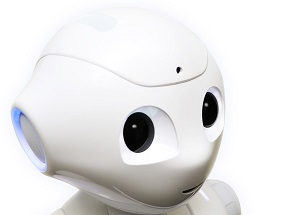
\includegraphics[width=0.5\textwidth]{chap06/text06-img001.jpg}
    \caption{Pepper (softbank)}
  \end{figure}
\end{frame}

\begin{frame}
  \frametitle{Open JTalk}
  \begin{itemize}
    \item 音声合成のためのソフトウェア
    \item 文字(テキスト)を読み上げる
  \end{itemize}
  \centering
  \includesvg[width=0.8\textwidth]{chap06/text06-img011.svg}
\end{frame}

\begin{frame}
  \frametitle{音声認識}
  \begin{itemize}
    \item 人間の声をコンピュータに認識させること
    \item 話し言葉から文字列への変換
    \item 音声の特徴を捉える
  \end{itemize}
  \note{画像を挿入}
\end{frame}

\begin{frame}
  \frametitle{Julius}
  \begin{itemize}
    \item 音声認識のためのソフトウェア
    \item 音声を聞き取って文字に変換する
    \centering
    \includesvg[width=0.8\textwidth]{chap06/Julius.svg}
  \end{itemize}
\end{frame}

\begin{frame}
  \frametitle{問題を解こう}
  \begin{itemize}
    \item 教科書2ページ 問題6-1
    \item 教科書2ページ 問題6-2
  \end{itemize}
\end{frame}

\begin{frame}
  \centering
  準備
\end{frame}

\begin{frame}
  \frametitle{ヘッドフォンをつけよう}
\end{frame}

\end {document}
